\section{LSST Phase 1 Science Roadmap - Bulge subgroup v1.0, August 2013}

Summary: This is version 1.0 of the LSST Bulge Science Phase 1 Roadmap. The Phase I document should identify the technical and scientific challenges for LSST Bulge work (without going overboard on the science) and to start to identify tasks for collaboration members in order to overcome these challenges on a timescale of a few years. 

Based on input from the Bulge subgroup, we have identified a number of technical issues that are important to Bulge science with LSST. We also highlight some suggested investigations - mostly based on simulation and archival work - that we believe would allow LSST to become a unique machine for conducting scientific discovery about the Milky Way Bulge. This document is organized as follows: 
\begin{enumerate}
\item Summary of Bulge LSST Science goals and match to LSST capabilities
\item Main technical issues these goals bring up 
\item Investigations that should be performed / questions to answer at this stage. 
\item Questions already arising for LSST development team 
\item References cited 
\item Figures 
\item Appendix: more detail about the Bulge LSST Science goals 
\end{enumerate}

A note on editing: Feel free to email either the subgroup leads (Will Clarkson and Victor Debattista; 
wiclarkson@gmail.com and vpdebattista@gmail.com ) or the mailing list (lsst-milkyway-bulge@lsstcorp.org ) with suggested edits. 

\subsection{Overview of LSST Bulge science goals}

These are kept deliberately broad at this stage (see Section 7 for more information), but point to the unique strengths of the Bulge as a test-case for Galaxy formation models: 
\begin{enumerate}
\item Detailed balance of populations as traced by morphology, chemistry, kinematics and distance 
\item The present-day mass distribution of the inner Milky Way as traced by Bulge star motions 
\item Wide-field examinations of other sub-populations and objects of interest. 
\end{enumerate}

\subsection{Match to LSST capabilities}
If the numbers in Ivezic et al. (2008), the Science Requirements Document (SRD) and the LSST Science Book are realized for the Bulge populations of interest, these three science goals should be within the capabilities of LSST. For reference, those numbers are: 
\begin{itemize}
\item Relative photometry: 5 mmag per-measurement rms (g,r,i), perhaps 50\% larger for u,z,y (SRD Table 14) 
\item Absolute photometry: 10 mmag per-measurement rms, color zero-points accurate to 5 mmag rms (SRD 
Tables 15, 16) 
\item Relative astrometry: 10-15 mas per-measurement rms depending on separation (SRD Table 18) 
\item Absolute astrometry: 50 mas per coordinate (SRD Table 20) 
\item Pixel-scale and seeing: Pixel-scale $\le$ 220 mas; at airmass 2, 
seeing-error 0.5 arcsec ($\gtrsim$ 2.3 pix; SRD 
Tables 10,11) 
\item Shortest possible exposure time: 5 sec, stretch-goal 1 sec (SRD Table 8) 
\item{At r=20, predicted performance when measurements are combined over the 10-year baseline survey:
\begin{itemize} 
\item Proper motion accuracy: 0.14 mas/yr, Photometric error 0.005 mag (single-visit), 0.003 mag (stack) 
\item These numbers come from from Table 6.6 and Figure 6.26 on Pages 193-195 of the LSST Science Book, v2. 
\item Note that the 10-year baseline survey is likely to be rather more generous than Bulge observations (by a factor of several - see Section 2.3). 
\end{itemize}
}
\item{For context, here are approximate apparent magnitudes for bulge populations of interest: MSTO roughly r$\sim$19.5 (r-band absolute magnitude about 4.0, plus distance and extinction), Red Clump giants roughly r$\sim$7.0 Note, however, that variations in the line of sight distance and extinction significantly broaden the observed distribution (X-shape alone leading to variation by 0.5 magnitudes or more; e.g. Saito et al. 2011). }
\end{itemize}
However, most of the Bulge populations of interest are more crowded than the baseline LSST survey to which the 
above numbers apply (Section 2.1 and Figure 1). 
While a seeing-limited large-scale survey like LSST is likely to be transformative for Bulge science, to reach these science goals we do need to understand how the LSST performance numbers change towards the Bulge, and what strategy will successfully overcome any limitations of the current reduction plans. 

\subsection{Leading Technical Issues}

\subsubsection{LSST as complementary to Gaia towards the inner MW}
LSST is supposed to smoothly extend the error-vs-magnitude curve of Gaia to fainter magnitudes (Ivezic 2008). Here are summary numbers for GAIA (de Bruijne et al. 2012 and Brown 2013), which are a bit more generous than Reyle et al. (2008; Figure 1). 
\begin{itemize}
\item Gaia Astrometry OK up to about 1 million stars / sq. deg., corresponding to about 278 stars per square arcmin. 
\item Gaia Photometry OK up to about 200 stars per square arcmin 
\item Gaia Spectroscopy OK up to about 10 stars per square arcmin 
\item Brown (2013) indicates $\sim$800 stars / sq. arcmin “can be dealt with” - what does this mean for actual 
precisions in this regime? 
\end{itemize}

For non-crowded regions (e.g. Science Book p193-195), LSST’s precision starts to exceed Gaia’s 
precision at r$\sim$~19.5 or so, comparable to the MSTO and sufficient to well-characterise 
red-clump giants already. 
However, this is unlikely to be realized in 
practice due to crowding; the GAIA - LSST handover magnitude may be somewhat brighter. 
\begin{itemize}

\item Gaia performance: What will the true performance of Gaia be towards the MW Bulge in reality? See e.g. Figure 1. 
\item Gaia/LSST magnitude boundary: In crowded fields, at what apparent magnitude will Gaia’s performance degrade and LSST be expected to “take over?” Is this transition magnitude fainter than, say, the fainter Red Clump Giants (RGC)s in most Bulge fields? 
\item Gaia’s observing strategy: For those objects within Gaia’s magnitude range of accuracy, how does Gaia’s observing cadence map onto the science goals for LSST Bulge work? 
\item Gaia and LSST in overlapping brightness ranges: For the brightness interval in which Gaia and LSST overlap in coverage, what will LSST add to those objects? Should observations in this overlap magnitude range be scheduled for cross-calibration, in the crowded fields towards the Bulge? 
\end{itemize}

\subsubsection{Crowded-field Photometry and Astrometry}
 This was perhaps the most common technical response in the Survey amongst MWLV members! 
The performance specifications in the Ivezic et al. (2008) survey document and the SRD, are for regions that are not too crowded, although it does not appear that 
the collaboration has yet reached official consensus on what "crowded" really means. At the moment, the rule of thumb appears to be 
about 200 stars per square arcmin. 
This limit is reached before the Main Sequence Turn-Off in many fields 
towards the bulge (Figure 1).
 
Thus, reaching the MSTO will likely require pushing LSST's photometry and 
astrometry software to regions that are much more crowded than LSST’s existing analysis stack was built to handle. Arising from this: 
\begin{itemize}
\item What measurement approaches will work best for LSST Bulge crowded fields? 
\item{Is rapid turnaround important for LSST Bulge photometry, or is a careful, if slower, analysis (taking, say, 
a few weeks to process) appropriate? }
\item Is rapid turnaround important for LSST Bulge astrometry? 
\item{In what mode will crowded-field work be performed? Do we require optional tools that would be run on 
specific small regions, or is it essential instead to produce the photometric and astrometric catalog for 
all regions observed, no matter how crowded? }
\item{What is the limiting depth required by the LSST Bulge science goals? To what source density (e.g. stars 
per square arcmin) does this correspond in real Bulge fields? }
\item{Conversely, if we assume the baseline analysis software that will deliver photometry and astrometry for 
regions $<$ 200 stars / sq. arcmin, how does this impact the Science Goals? See e.g. Figure 1 in Section 6 
below.}
\item{If any science goals are precluded under the baseline scenario, does their resurrection deliver science of 
sufficient import to justify the extra effort developing crowded-field analysis tools? }
\item{
The LSST planning software already includes sophisticated tools to simulate stellar populations in the 
inner MW (its crowding predictions towards the plane were used to set the galactic latitude limits for the main LSST survey). How well do the predictions of these tools match reality? Are their predictions too conservative? }
\item{One survey respondent recommended that astrometry not be treated as an afterthought, but be built in to analysis tools as a key requirement. }
\end{itemize}

\subsubsection{Observation setup (including total time, saturation issues)}
How do the different science goals interact with each other when designing observations? Are some science cases excluded by others? 

\begin{itemize}
\item{Total observing time: Based on a quick query of OpSim (performed in June 2012), bulge fields were slated to receive ~one fifth the number of pointings per field when compared to the baseline survey (Figure 2). Assuming those numbers are still current, now is the time to advocate for a more suitable strategy. In particular: 

\begin{itemize}
\item{Lower number of exposures per field is probably unimportant for deep stacks since the crowding is higher than baseline anyway. }
\item{ However, for investigations requiring multiple exposures whatever the depth (e.g. proper motions, monitoring variable-object standard candles), the reduced total number of observations might prevent the desired science goal being reached. }
\item How should observations be distributed along the total time allocation to maximize the science? 
\item How many pointings per object are needed for a given science case? 
\item Is there a strong enough case to request a larger total allocation time? 
\item{Saturation issues: What range of exposure times will allow both the bright and faint objects to be 
covered in the same campaign? What is the observing duty cycle as a function of exposure time? At what 
(if any) instrumental magnitude do persistence effects set in? }
\item{
Cadence: How do the cadence requirements for the different science cases interact with each other? For 
example, can variable-object standard candles with very long periods (hundreds of days or longer) be monitored in an observing program that also seeks short-period variables? In this example, if (say) a logarithmic cadence strategy is adopted, does this preclude other science? }
\item{What happens if the total allocation for Bulge science is reduced? Do we need to produce a contingency plan in this case? }
\item{Extinction and filter choice: Will extinction-correction rely on cross-matching to catalogs at other wavelengths? Or, does the requirement to correct for extinction drive a minimum number of filters for every observation? }
\item{Astrometry and filter choice: The Science book (Section 3.7) seems to suggest that the (r, i) filters will be best for astrometry. To pursue bulge astrometry, should a separate set of observations in a smaller number of filters be taken? }
\end{itemize}
}
\end{itemize}

\subsubsection{Calibration and calibration products}
\begin{itemize}
\item What calibrations do we (the investigators) need to conduct our own specialized analyses of favorite 
regions? 
\item How will calibration products be made available to the community? 
\item{For how long and in what format will supporting observational telemetry (e.g. telescope temperature, 
observed seeing, etc.) be maintained? WIll this be available to the investigator? }
\end{itemize}

\subsection{Investigations suggested for LSST Bulge science}
The above considerations suggest the following investigations. We are aware that in several cases this might be as quick as a literature or archive-search. 
\subsubsection{Simulation}
Baseline capability of LSST in crowded fields with the currently-planned measurement software: 
\begin{itemize}
\item{Simulate observations towards a variety of regions towards the Bulge, at a variety of exposure-times, 
with input properties of interest (e.g. variability, proper motion, extinction), and attempt to recover these using the existing software stack. }
\item{Use this to estimate random and systematic effects on photometric and astrometric completeness and precision as a function of the stellar crowding. }
\item{This dataset might already exist - were these simulations performed to set the Galactic Plane avoidance limits for the baseline survey already? }
\end{itemize}

\subsubsection{Simulation + Archive}
Science impact of crowding limit: Using crowding limits obtained from 4.1 above or otherwise, examine available source-catalogs towards the bulge to determine, under those crowding limits: 
\begin{itemize}
\item What is the region of avoidance with current LSST software, in galactic coordinates, as a function of magnitude? 
\item What stellar populations in and towards the bulge become unavailable using this limitation? 
\item What science does this preclude? 
\end{itemize}

\subsubsection{Simulation}
Observing strategy for saturated objects in crowded fields: 
\begin{itemize}
\item{Simulate observations for a well-chosen sample of fields towards the Bulge, at a range of exposure times 
from 1s to 15s, to estimate: 
\begin{itemize}
\item What range of exposure times is needed to attain high-precision measurements of the bright 
stars in the field of view? 
\item What artefacts are bright objects expected to produce in the longer exposures, and how can 
their effects be characterized and mitigated? 
\item How do measurement systematics vary with exposure time? 
\item What is the tradeoff between observing efficiency and exposure time? 
\end{itemize}
}
\end{itemize}

\subsubsection{Literature, Simulation, ground-based data}
Performance of existing crowded-field photometry and astrometry tools on likely LSST observations towards the Bulge: 
\begin{itemize}
\item How do existing crowded-field measurement techniques scale to LSST-like applications? 
\item{What scale of simulation is practical before LSST goes on-line? Can we expect to run a complete suite of 
imaging-sets under a variety of reduction strategies? }
\item{How do changes to analysis software fit in with the LSST software pipeline as it currently exists? }
\end{itemize}

\subsubsection{Simulation combined with existing data and archives): Fidelity of LSST’s simulation software applied to Bulge regions: }
\begin{itemize}
\item{Compare LSST simulation predictions with existing datasets towards the Bulge to determine how well these simulations reproduce actual data. }
\item{A large number of potential comparison datasets, from broad-shallow to narrow-deep}
\item{The ImSim/OpSim team might already be doing this... }
\end{itemize}

\subsubsection{(Simulation, literature, archives): Harder numbers for science requirements: }
\begin{itemize}
\item{
Use existing archives / literature to map figures of interest across the bulge region (e.g. number of stars 
per square arcminute down to a limiting depth as a function of apparent magnitude and color). Do this 
for several populations of interest (e.g. Red Clump Giants). }
\item{Modeling: To make further progress on (for example) mass models of the Bulge, what size of tracer-star 
sample is needed? }
\item{Modeling: Under the current best bulge models, what is the prediction of proper motion as a function of 
line of sight distance for sight-lines towards the bulge? What does this imply for proper motion precision requirements? }
\end{itemize}


\subsubsection{(Simulation): Observing strategy to best meet science goals: dithering, pointings}
\begin{itemize}
\item{Simulate observations with different dithering strategies to determine the best strategy under likely time 
allocations.}
\end{itemize}

\subsubsection{(Archive, Simulation): Appropriateness of existing catalogs for LSST Bulge operations: }
\begin{itemize}
\item{Determine to what extent successful observations require information from external catalogs to succeed. 
Determine how the quality of these catalogs changes over the Bulge, and thus what (if any) effect variation in external catalog quality will hinder science observations towards the Bulge. }
\end{itemize}

\subsubsection{Literature, personal communication): Complementarity to GAIA }
\begin{itemize}
\item{Find out the current best estimate for GAIA’s performance towards the Bulge. Do hard numbers exist from 
the GAIA team for what happens to GAIA’s astrometric and photometric precision in highly crowded regions? What did Brown (2013) mean by “[$\sim$800 stars/sq arcmin] can be dealt with”? }
\end{itemize}

\subsubsection{(Observation, archive): Precursor data }
\begin{itemize}
\item{Determine what precursor data already exists to answer the questions raised in this document. }
\item{As a sub-group, if necessary regions of parameter-space are NOT probed by these observations, 
determine a consensus plan to apply for further precursor data. }
\item{We want to avoid the situation where members of the LSST Bulge sub-group submit proposals 
that compete with each other for similar precursor data. }
\end{itemize}

\subsection{Questions and wishlist arising for those developing the LSST facility and its software}
\subsubsection{Existing simulations: }
\begin{itemize}
\item Improved knowledge desired on how to access simulated datasets. 
\end{itemize}

\subsubsection{Running custom simulations }
\begin{itemize}
\item What computer hardware is required to run LSST simulations? 
\item{What is the key factor determining the variation of time elapsed for a simulation on the same hardware 
-- the total number of sources, or something else? }
\item{Tutorials are desired on how to set up and run the simulation software. }
\end{itemize}

\subsection{Existing and planned analysis software }
\begin{itemize}
\item Tutorials on the Data Management system 
\item{Detailed understanding of the uncertainties (their production and propagation) through the LSST 
simulations and measurement routines }
\item{Tutorial on running the LSST pipeline on non-LSST data }
\item{What are the current capabilities of point-source software for LSST? What are its limitations (e.g. 
maximum array-size)? }
\end{itemize}

\subsubsection{External catalogs for LSST photometry }
\begin{itemize}
\item How reliant is LSST calibration on cross-matching to external catalogs? 
\item What capabilities for cross-matching with external catalogs, can we expect? 
\item{ Bulge regions may have more sources per square arcmin than typical for the baseline survey. How does 
the time required to crossmatch scale with catalog size? How are multiple possible matches handled? }
\end{itemize}

\subsection{References cited: }
%%\begin{verbatim}
%%1. Brown 2013: http://www.strw.leidenuniv.nl/~brown/gaia/gaia­dpac­overview.pdf 
%%2. de Bruijne et al. 2012: http://adsabs.harvard.edu/abs/2012Ap%26SS.341...31D 
%%3. Howard, C. D. et al. 2009 ApJ 702, L153 
%%4. Ivezic, Z. et al. 2008 http://arxiv.org/abs/0805.2366 
%%5. Nidever, D. L. et al. 2012 ApJ 755, L25 
%%6. Reyle, C. et al. 2008: http://arxiv.org/abs/0812.3743v1 
%%7. Saito, R. 2011 AJ 142, 76 
%%\end{verbatim}

\subsection{Figures }

\begin{figure}[h]
    \centering
    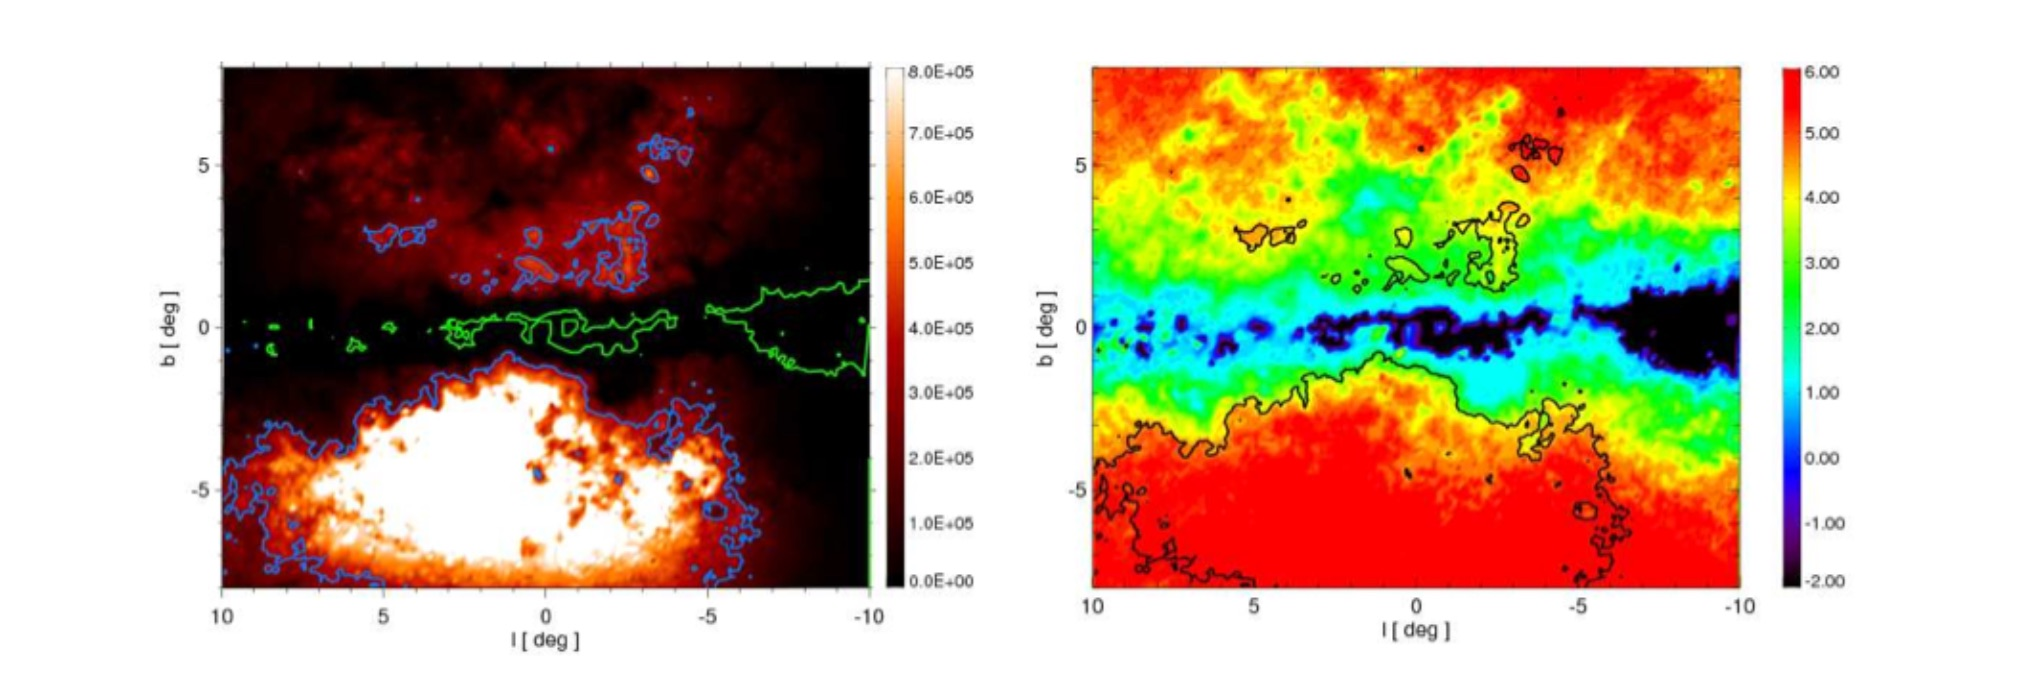
\includegraphics[width=1.0\textwidth]{bulge_fig1a.jpeg}
    \caption{\label{fig:bulge1a}
Figure 1a: This shows predictions of the Besancon model for the inner Milky Way, in the context of GAIA’s performance estimates as of 2008. The left-hand panels show spatial density (stars per sq. deg.), the right shows the absolute magnitude (in G-band, approx SDSS r) of stars just reached at their assumed limiting magnitude. This figure shows GAIA’s astrometric fields (the GRP and GBP instruments – limiting magnitude G=20). The blue contour shows the iso-density of 600,000 stars per square degree (167 stars per square arcminute, or a little less 
crowded than LSST’s baseline limit at present). The green contour shows the iso-density of 100 stars per square degree, or 0.028 stars per square arcminute. Notice that in G-band, it is the bright area away from the plane that is in the region of avoidance, not the dark area covering the plane itself. This is Figure 3 of Reyle et al. 2008. }
\end{figure}

\begin{figure}[h]
    \centering
    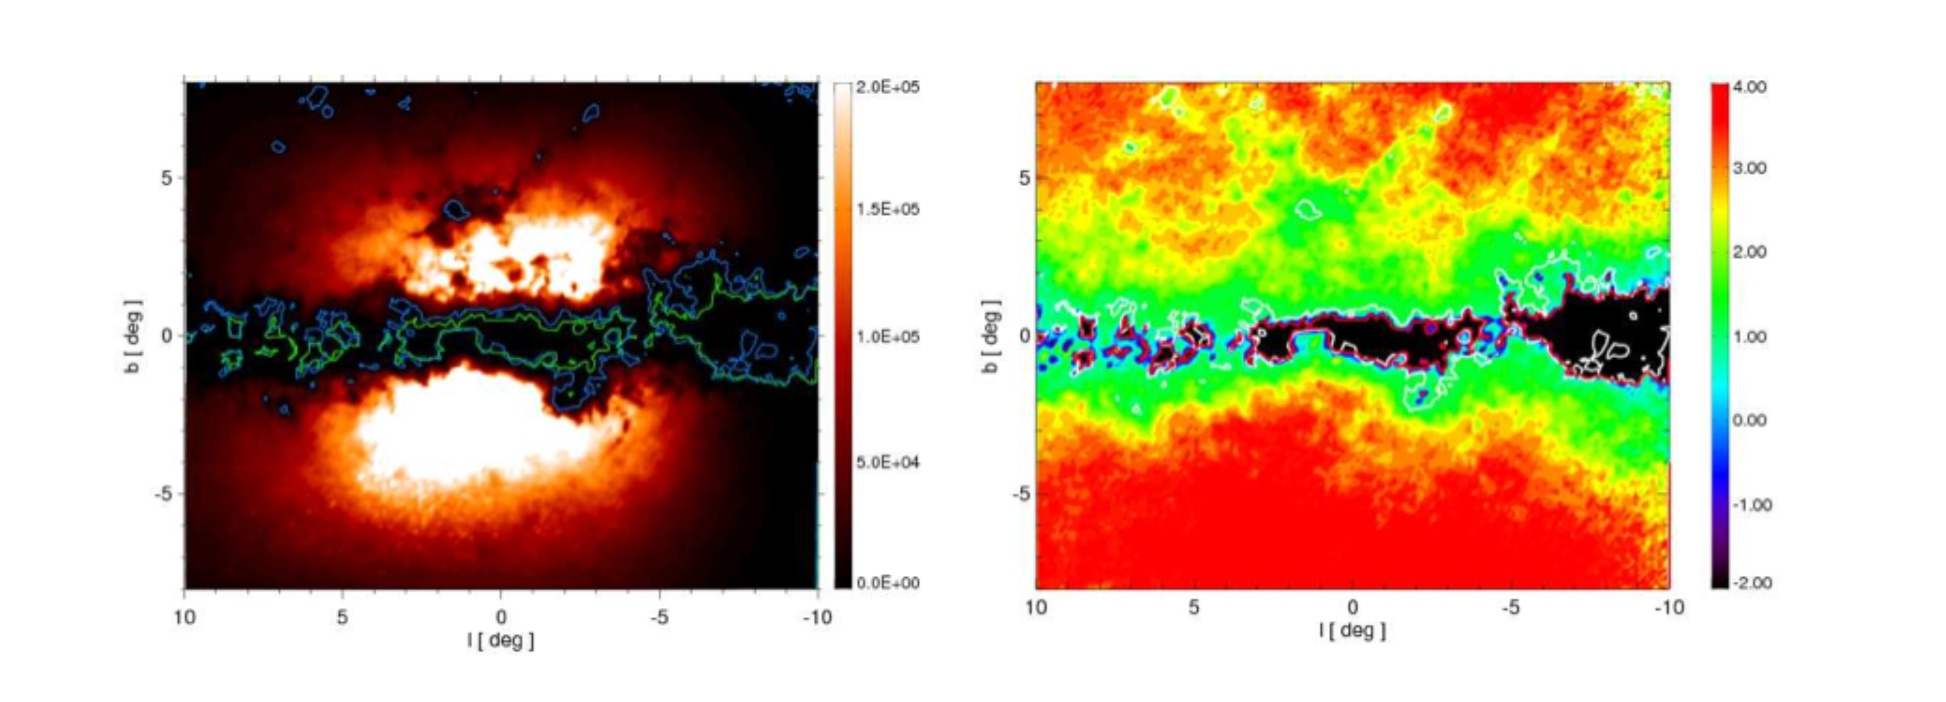
\includegraphics[width=1.0\textwidth]{bulge_fig1b.jpeg}
    \caption{\label{fig:bulge1b}
Figure 1b: As Figure 1a, this time for GAIA’s spectrometer (RVS). This instrument has limiting magnitude G=17 and a much more stringent crowding limit: 30,000 stars per square degree, or about 8.3 stars per square arcminute. With these performance numbers, only the very inner (extincted) plane is accessible to GAIA’s RVS spectrometer. This is Figure 4 of Reyle et al. 2008. }
\end{figure}

\begin{figure}[h]
    \centering
    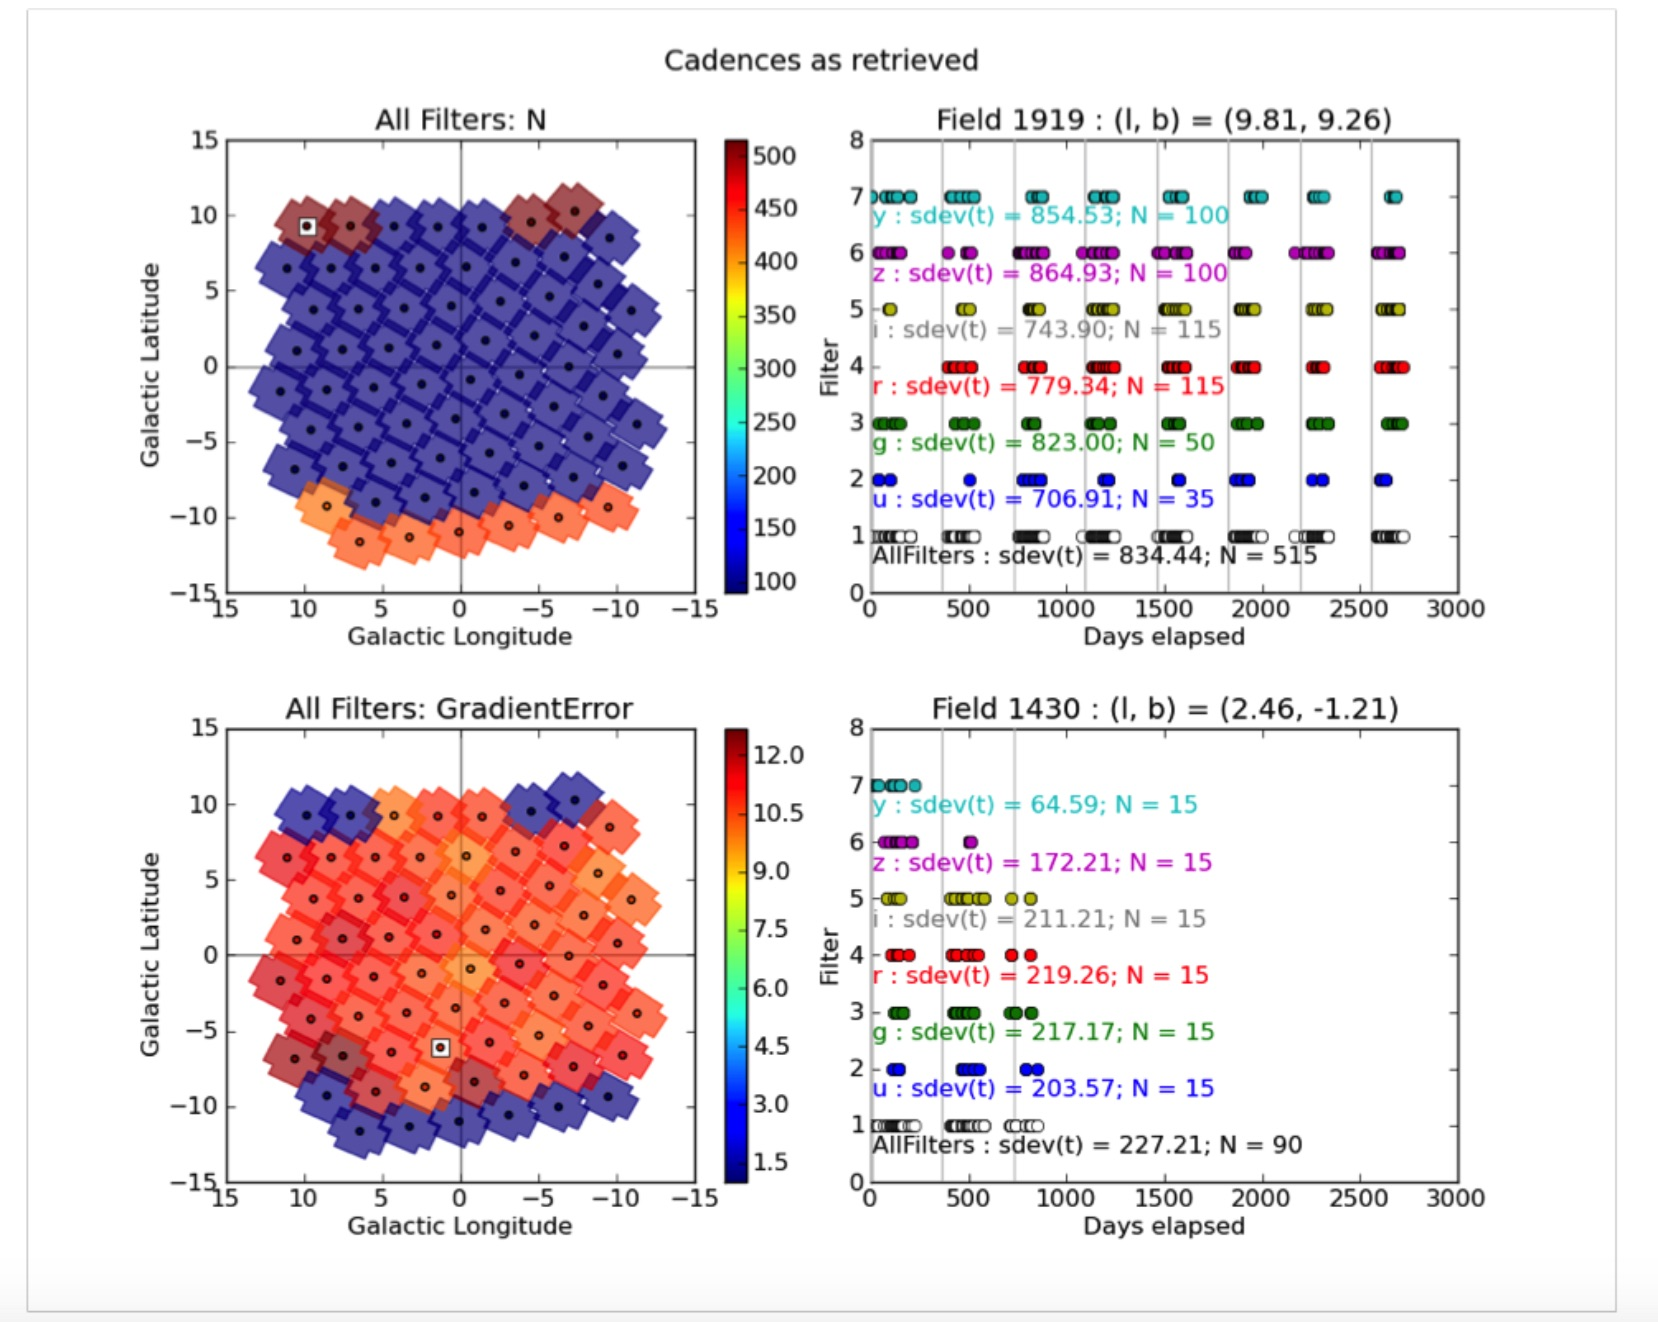
\includegraphics[width=1.0\textwidth]{bulge_fig2a.jpeg}
    \caption{\label{fig:bulge2a}
Figure 2a: This figure shows a basic example of the kind of strategy assessment that could be performed to optimize observations. OpSim was queried for all regions close to the galactic center (-15 < l < 15 degrees) using OpSim as of June 5th 2012, and the dates of all retrieved observations were used to estimate the impact of proper motion measurement due to time allocation and the concentration of observations under the retrieved strategy. Top-left: Map of fields in galactic coordinates, color-coded by the total number of observations per field. 
Bottom-left: Map of fields, this time color coded by the formal error on proper motion based on the samplings retrieved from OpSim. Top-right and Bottom-right show time-series for the samplings for example fields (top = baseline survey, bottom = example bulge field) under the OpSim strategy at the time. All else being equal, the proper motion precision for the Bulge strategy at the time is a factor ~8 worse than the baseline survey just by virtue of the lower time allocation and its concentration, but there are obvious steps that could be taken to improve matters (such as spreading the same observations over the full time baseline of the survey). }
\end{figure}

\begin{figure}[h]
    \centering
    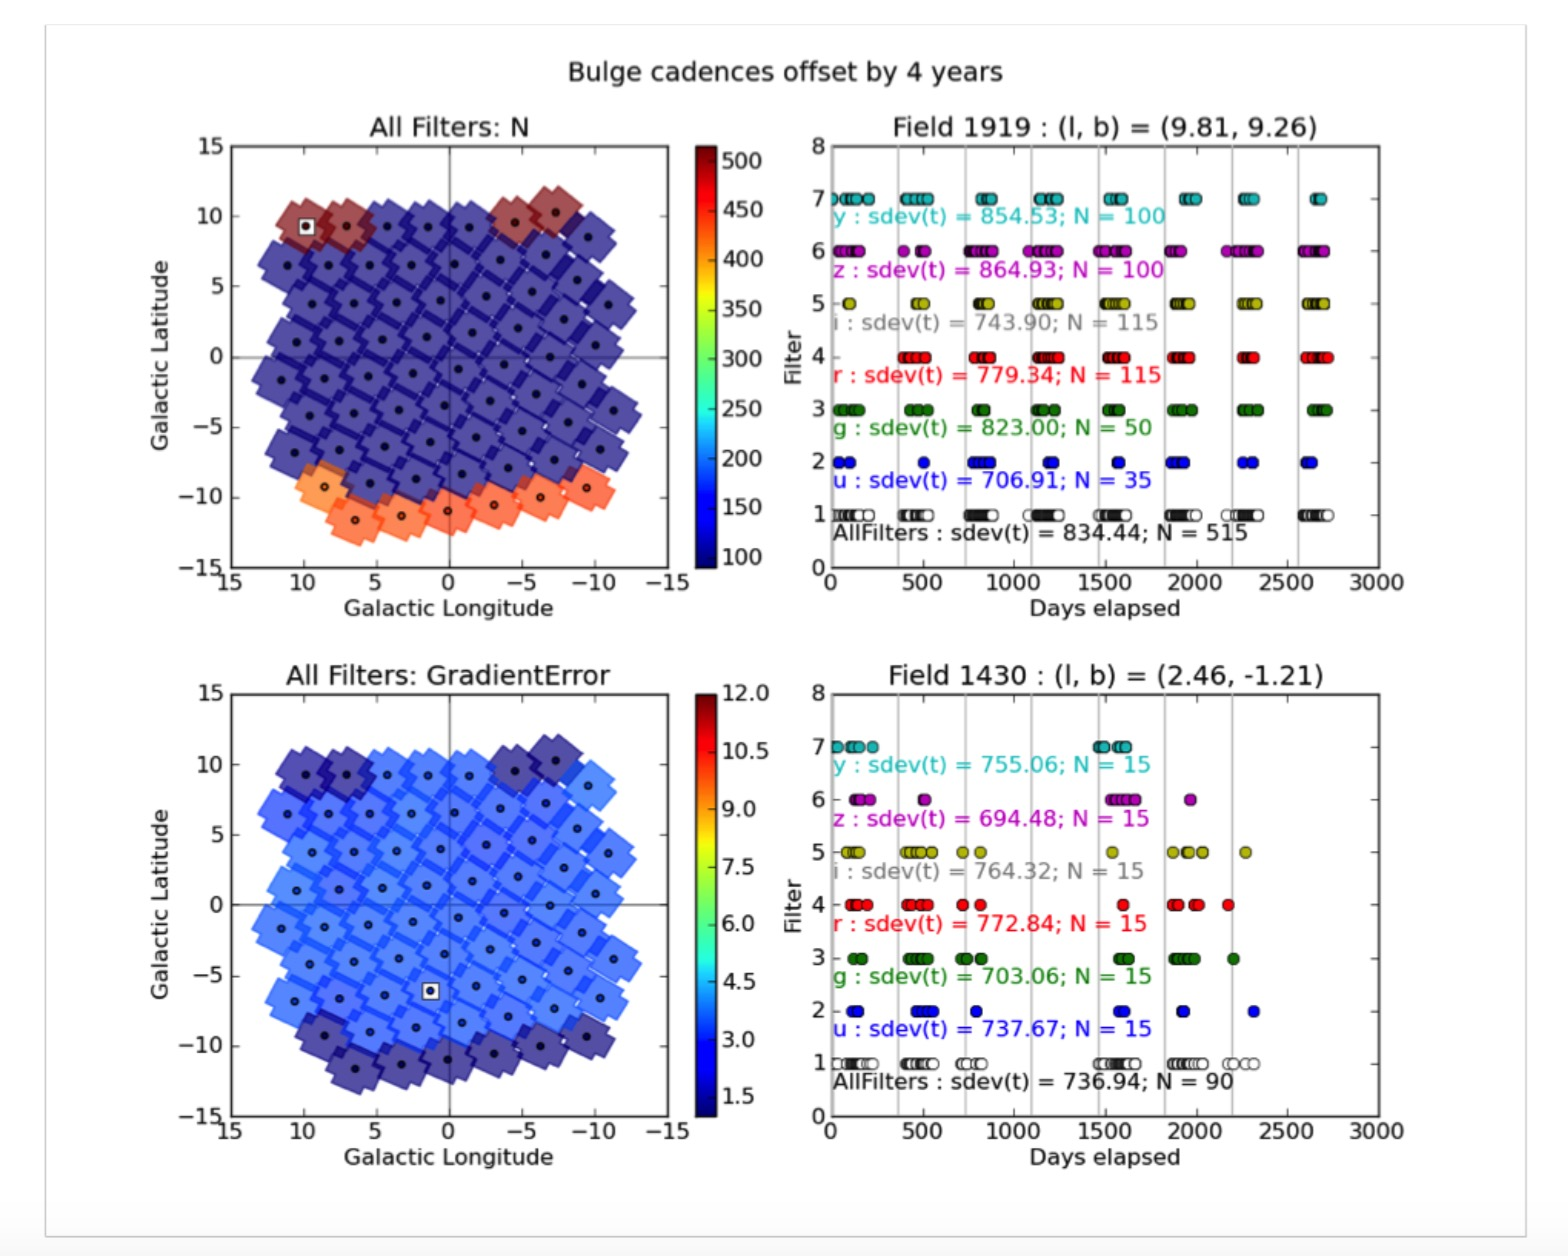
\includegraphics[width=1.0\textwidth]{bulge_fig2b.jpeg}
    \caption{\label{fig:bulge2b}
Figure 2b: As Figure 2a, this time with the original Bulge allocation spread along the same time interval as the baseline survey (note the total number of exposures for the Bulge is the same as for Figure 2a). The formal gradient error has already been reduced significantly, to a factor ~2-3 over the baseline survey. }
\end{figure}



\subsection{Appendix}
more detail about LSST Bulge science goals: To keep the focus of the Phase I document on technical investigations to be performed, much of the detail on the science goals in v0.2 has been moved here. Goals: 
i. Detailed balance of populations as traced by morphology, chemistry, kinematics and distance: 
\begin{itemize}
\item{Morphology: Uniform, accurate positions and magnitudes across sufficiently wide field to characterize 
X-shaped structure. Depth: at least 2 magnitudes below the red clump giants, and ideally down to the 
Main Sequence Turn-off (MSTO). }
\item{Chemistry: Multi-color photometry, with uniformly calibrated photometric zeropoint in each region and 
filter. Depth as per Morphology. Cross-match with NIR catalogs (e.g. 2MASS, particularly VVV) to account 
for interstellar absorption. }
\item{Kinematics, particularly membership probabilities: Tracer stars (e.g. the Red clump giants) may overlap 
significantly with existing and planned spectroscopic catalogs. However, proper motions from LSST itself should allow all stars to be assigned membership probabilities. Requires proper motion precision better than 1 mas / yr, and ideally better than 0.5 mas/yr. }
\item{Distance: Photometric variability will allow standard candles (including but not limited to RR Lyraes, eclipsing binaries) to trace the populations along line-of-sight distance. Requires monitoring cadence sufficient to characterize these tracers. }
\item{Bulge, Thick Disk, inner halo, and Sgr Dwarf: A uniform multiband survey with high astrometric quality that spans the entire inner Galaxy will offer the quantitative means to define how the bulge is related to the inner disk and halo, and to settle whether any “classical” spheroidal-like bulge is separable from the bar. The complexity of the Sgr dwarf populations can be separated from the generally much closer Galactic populations. }
\end{itemize}

ii. The present-day mass distribution of the inner Milky Way (MW), as traced by the Bulge star motions: 
\begin{itemize}
\item{Proper motions: Produce a catalog of proper motions accurate to <1 mas/yr (ideally <0.5 mas/yr) for all 
objects down to the MSTO. Use the wide-field, multi-sight-line nature of this catalog to test models of bulge formation and evolution. E.g. what size of "classical-bulge" population is consistent with the observed velocity dispersion as a function of position and depth? Are the putative kinematic substructures (e.g. Nidever et al. 2012, see also Howard et al. 2009) real? What is the total mass felt by Bulge stars, as a function of cylindrical coordinates (R, theta, phi)? Requires carefully-designed survey strategy. }
\item{Line-of-sight motions: Merging with existing and planned spectroscopic catalogs 3D measured motions for a massive sample of Bulge stars.}
\end{itemize}

iii. Wide-field examinations of other sub-populations and objects of interest: 
\begin{itemize}
\item{Tidal streams and kinematic substructures that pass through the inner MW: With such a wide-field catalog, 
LSST should provide important tracer information for merger remnants and other discrete features in 
phase-space.}
\item{How many Globular Clusters (GCs) exist in the inner MW? VVV is already uncovering more GCs in the inner 
MW, what scientific investigations will LSST enable for these objects? }
\item{
Hypervelocity stars: Observe rare, fast-moving objects ejected from the very inner MW, and use them to 
constrain stellar formation and ejection processes near Sgr A*. }
\item{Is there a “nuclear” population? }
\end{itemize}


